\documentclass{article}
\usepackage[utf8]{inputenc}

\usepackage{float}
\usepackage{natbib}
\usepackage{graphicx}
\usepackage[export]{adjustbox}
\usepackage{multirow}
\usepackage{hyperref}
\usepackage{titlesec}
\usepackage{ragged2e}



\begin{document}
\title{COS301 Team Gamma: Notification Team Goals}
\begin{figure}
    \centering
    
\includegraphics[width=\textwidth]{logo.png}
\end{figure}
\date{March 2020}

\maketitle

\section{Introduction}
This document describes the responsibilities and all deliverables for the \\ Notification Team.
\\ \\
Demo \#1 Due Date: Thursday 12 March 20:00
\newpage

\section{Organisation}
\subsection{ClickUP}
You need to elect a team leader if you have not done so already. Work together with this member to create tasks and sub-tasks for each member in your team on \url{http://clickup.com} (on the COS301 workspace you have been invited to). \\

\begin{figure}[h]
    \centering
    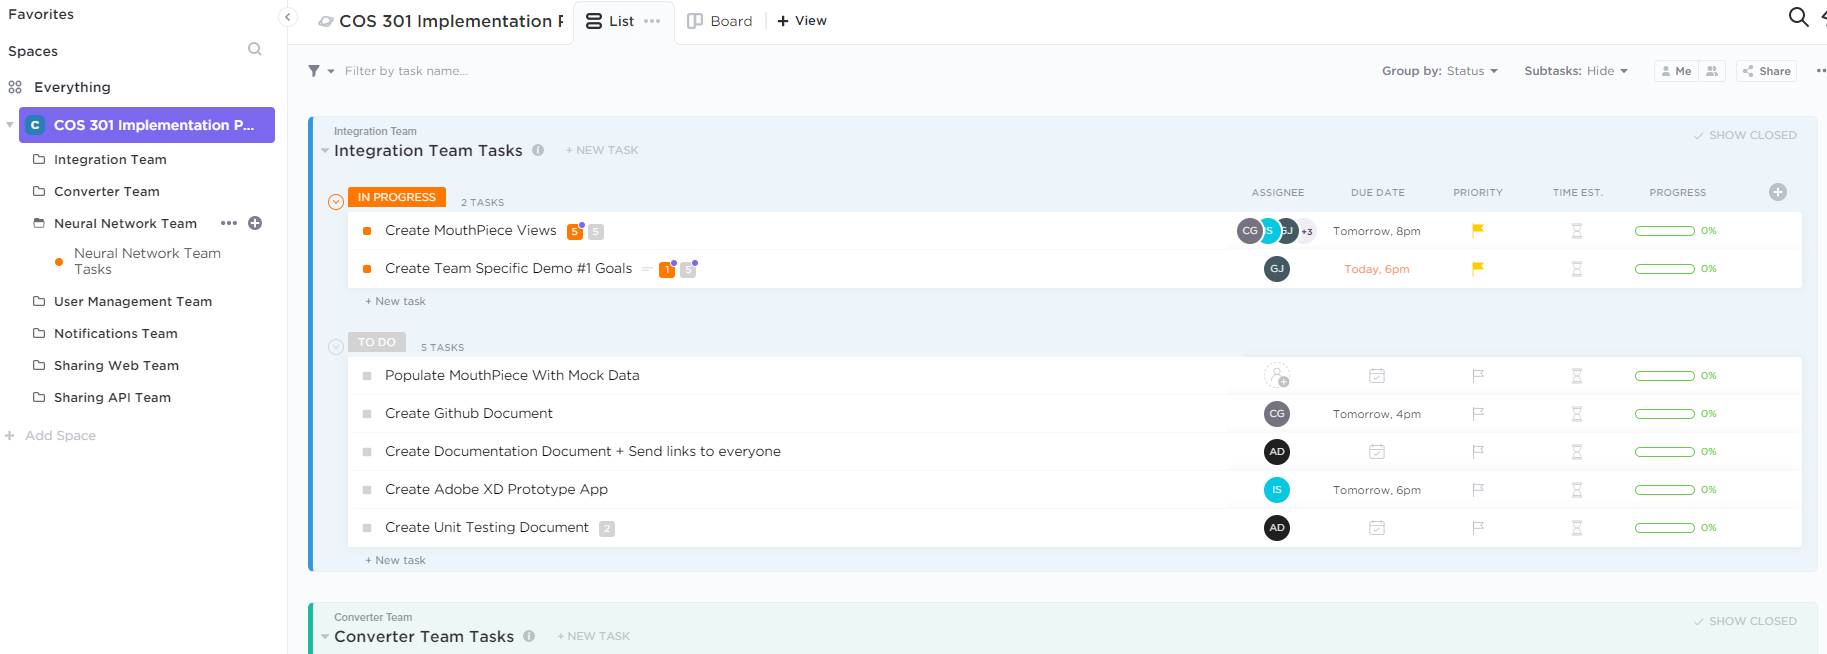
\includegraphics[width=\textwidth]{clickup.png}
\end{figure}

Ensure that you indicate progress and mark tasks as complete. This page will be displayed at the demo.

\subsection{Slack}
Although we have created a WhatsApp group - we do still find it easier for in-group discusions to happen on the slack channels. Simply login to \url{http://cos-301.slack.com}

\newpage

\section{Overall Team Tasks}
These are the tasks to be done by your team for the final product (not specifically Friday's demo).

\begin{itemize}
    \item Implement the triggers to send different types of notifications (through the Android App, SharingAPI (PHP) and UserManagementAPI (PHP)
    \item Send Local push notifications: e.g. “Did you know that you can upload your own designs on our website” trough Android App (in Flutter)
    \item Send Network push notifications: e.g. “10 new mouths have been uploaded - check them out!” via SharingAPI (in PHP, via Google Firebase API)
    \item Send Email notifications: “You have successfully registered for MouthPiece” via UserManagementAPI (in pure PHP, using local mailserver)
\end{itemize}

\vspace{1cm}

\begin{center}
   \textit{The tasks are always subject to change, but we have tried our utmost best to sketch out the entire project ahead.}
\end{center}

\newpage


\section{Team Tasks for Friday}

\subsection{Documentation}
\textbf{All documentation to be created in Overleaf} - Overleaf link to be sent to the Integration Team

\subsubsection{Implementation Plan}
Create a document explaining different examples of notifications that you will send for each category of notification (expand on the examples above) \\

\textbf{Futhermore:}
\begin{itemize}
    \item List the technologies that you will use (explained above).
    \item Draw basic flow diagrams on \url{http://draw.io} explaining how the notifications get sent (through which systems, APIs, on which triggers etc) and attach these to the Overleaf document.
\end{itemize}

\subsubsection{Frameworks}
You are required to do some research on frameworks that you could implement to assist your \textbf{Overall Team Tasks}. Write a short report on only the frameworks that you are keen to implement. Show its benefits and how you can implement it with the existing technologies. \\

\textbf{Some examples}
\begin{itemize}
    \item \url{https://pub.dev/packages/flutter_local_notifications}
    \item \url{https://firebase.google.com/docs/reference}
    \item \url{https://www.w3schools.com/php/func_mail_mail.asp}
\end{itemize}

\subsection{Development Environment}
You are required to setup the development environment (have it running on at least one member's device, ready to demo). Setup everything you think you require. \\
\newline
\textbf{At bear minimum}
\begin{itemize}
    \item Android Studio
    \item Visual Studio Code
    \item Flutter
\end{itemize}

\begin{center}
   \textit{This is required for your implementation in any case.}
\end{center}

\subsection{Hosting Environment}
Your team will already deploy your demo for Friday on the Apache web server. You will demo your FTP setup and showcase the live URL.\\

\textbf{Use the following FTP details:} 

\begin{itemize}
\begin{itemize}
\item Host: ftp.teamgamma.ga
\item Username: notification@teamgamma.ga
\item Password: SN8qbkwo0Z
\item Port: 21
\end{itemize}
\end{itemize}

\\
\begin{flushleft}
    Your FTP login details are rooted in: \url{http://teamgamma.ga/notification/}. i.e. any uploads will be visible on that URL. This will be moved to the SharingAPI and UserMangementAPI on final deployment.
\end{flushleft}

\textbf{Use the following email details:} 
\begin{itemize}
\begin{itemize}
\item Incoming Server: mail.teamgamma.ga (IMAP Port 993)
\item Outgoing Server: mail.teamgamma.ga (SMTP Port 465), Port 26 for non-SSL (try to use SSL if possible)
\item Username: mouthpiece@teamgamma.ga
\item Password: SN8qbkwo0Z
\item Port: 21
\end{itemize}
\end{itemize}


\begin{center}
   \textit{If you have any issues with the hosting, or require additional server resources, contact Giovanni (on Slack).}
\end{center}

\newpage

\subsection{Implementation}
\subsubsection{Notification Demo}
You are required to create two separate demo entities:

\begin{enumerate}
    \item You are required to setup a basic Flutter app (no interface required other than a hello world with a button). Then implement the \url{https://pub.dev/packages/flutter_local_notifications} or similar framework to send a local push notification on your device when the button is pressed. This needs to work offline and you will need to demo it on your actual device. 
    \item You are required to setup a simple PHP page (\url{http://teamgamma.ga/notification/index.php}) with a button which sends a predefined email body ("You have successfully registered for MouthPiece or similar..") to a predefined email address. The email needs to be sent through the mouthpiece@teamgamma.ga email. You need to deploy this on the Apache server (see: \textbf{Hosting Environment})
\end{enumerate}

\subsubsection{Unit Testing}
Describe how your team will implement unit testing. Better yet - implement it in the Demo where possible.


\end{document}